% English translation of the verified Chinese baseline. Structural identifiers must remain synchronized.
\section{Numerical Experiments and Results}\label{sec:numerical-results}

\subsection{Objectives, numerical models, and evaluation methods}\label{sec:numerical-6-1}

The numerical experiments successively examine the low-dimensional network implementation, learning behavior on a fixed \(N=2\) modal model, and consistency of the COMSOL--Galerkin canonical data mapping. P0 uses a four-dimensional nonlinear coupled oscillator to compare an unconstrained vector-field network, a Real HNN, a standard complex-linear CHNN, and a widely linear CHNN. P1, P1.5, and P1.6 use three fixed trajectories---mode1, mode2, and mixed12---to study derivative supervision, gray-box residual learning, and hard equilibrium constraints. Each test split holds out one complete trajectory, and the five random seeds represent algorithmic repetitions rather than independent physical samples. The canonical-data experiments isolate errors in coordinates, cotangent momenta, and generalized-force labels and assess the data-generation conditions needed for later multi-amplitude experiments.

The evaluation quantities include vector-field relative L2 error, rollout error, linearization error, energy drift, canonical closure error, and observed time-discretization order. The Bridge perturbation-energy criterion and the force-v2 joint-L2 criterion address energy drift and force closure, respectively, and use independent thresholds. Training, validation, and test data are partitioned by complete parameterized operating conditions rather than by random points from a shared trajectory. The full 96-trajectory data set, P2 model comparison, open-port analysis, high-fidelity discrepancy study, and numerical KAM validation remain subjects of subsequent numerical work; the present small-sample results are not extrapolated to those tasks.

\subsection{Numerical implementation and the COMSOL--Galerkin bridge}\label{sec:numerical-6-2}

The implementation was checked by source compilation, editable installation, component and interface tests, and a synthetic-data training workflow. Thirteen regression-test files were run in isolated processes for three consecutive rounds without failure. These tests assess software consistency rather than scientific model performance.

The COMSOL--Galerkin bridge comprises stationary exports, modal-reality checks on meshes 40 and 80, the first 12 production modes, and three \(1\,\mathrm{s}\) candidate trajectories. The original perturbation-energy criterion uses a \(0.5\%\) threshold and is met only by mode2; under the exploratory \(1\%\) threshold, all three trajectories satisfy the criterion. Force-v2 tests force closure on common-support indices \(2\ldots998\), with a fixed \(p[2]\) anchor and an independent \(2\%\) joint-L2 threshold; all three trajectories meet that criterion. \Cref{tab:bridge-gate-summary,fig:bridge-gate-separation} reports these tests separately so that the energy and force criteria are not conflated.

\begin{table}[htbp]
\centering
\caption{Trajectory-level comparison of Bridge perturbation energy and force-v2 force closure. Energy drift is evaluated against the \(0.5\%\) criterion and the exploratory \(1\%\) criterion; force-v2 uses an independent joint-L2 criterion.}
\label{tab:bridge-gate-summary}
\scriptsize
\setlength{\tabcolsep}{4pt}
\begin{tabular}{@{}lccccc@{}}
\toprule
Trajectory & Energy drift (\%) & \(<0.5\%\) & \(<1\%\) & force-v2 (\%) & \(<2\%\) \\
\midrule
mode1  & 0.815090 & fail & pass & 1.513677 & pass \\
mode2  & 0.329369 & pass & pass & 0.062551 & pass \\
mixed12 & 0.523328 & fail & pass & 1.080748 & pass \\
\bottomrule
\end{tabular}
\end{table}


\begin{figure}[htbp]
\centering
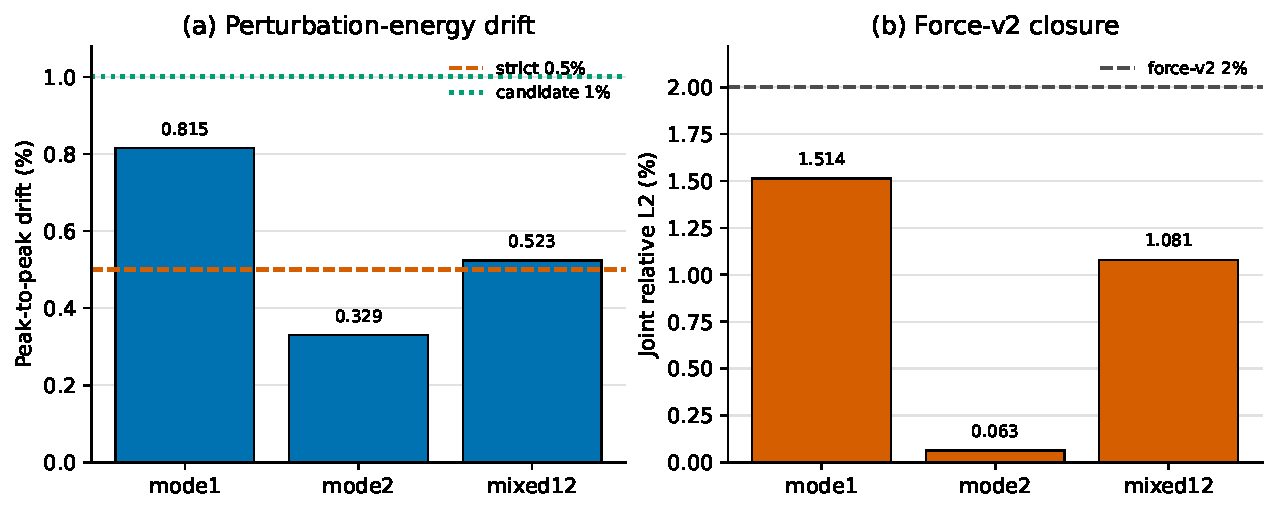
\includegraphics[width=0.94\linewidth]{figures/fig_bridge_gate_separation.pdf}
\caption{Bridge perturbation-energy criteria and the force-v2 force-closure criterion. The left panel applies the \(0.5\%\) criterion and the exploratory \(1\%\) criterion to the same perturbation-energy drift; the right panel shows the force-v2 joint-L2 error and its independent \(2\%\) threshold.}
\label{fig:bridge-gate-separation}
\end{figure}

\subsection{Identification results for the conservative branch}\label{sec:numerical-6-3}

\subsubsection{P0 low-dimensional architectural baseline}\label{sec:numerical-6-3-p0}

P0 uses \(80/16/20\) training/validation/test trajectories on the common four-dimensional coupled oscillator, with 80 steps per trajectory, \(\Delta t=0.025\), 300 epochs, and five algorithmic seeds. With the quadratic physics baseline included, the standard CHNN has vector-field and rollout relative L2 errors of \(0.0109144\) and \(0.0351959\), respectively, below the Real HNN values of \(0.0122422\) and \(0.0444270\). Its energy drift, \(0.00455759\), is not lower than the Real HNN value \(0.00402084\). This experiment therefore supports low-dimensional implementation and architecture comparisons but cannot replace a P2 comparison on COMSOL data or a KAM analysis.

\begin{table}[htbp]
\centering
\caption{Model comparison for the P0 quadratic-physics branch. The vector-field network does not use a physics baseline.}
\label{tab:p0-summary}
\small
\begin{tabular}{@{}lccc@{}}
\toprule
Model & Vector-field relative L2 & Rollout relative L2 & Energy drift \\
\midrule
Vector-field network & 0.0200837 & 0.103076 & 0.0245256 \\
Real HNN & 0.0122422 & 0.0444270 & 0.00402084 \\
Standard CHNN & \textbf{0.0109144} & \textbf{0.0351959} & 0.00455759 \\
Widely linear CHNN & 0.0121700 & 0.0458872 & 0.00403167 \\
\bottomrule
\end{tabular}
\end{table}


\subsubsection{P1, P1.5, and P1.6}\label{sec:numerical-6-3-p1}

All \(60/60\) P1 runs completed. Across the three held-out trajectories, the standard CHNN has joint vector-field relative errors of \(0.1417\%\)--\(0.2444\%\), rollout errors of \(0.2131\%\)--\(1.5237\%\), and linearization errors of \(0.3125\%\)--\(0.3286\%\). In the five-seed comparisons for this small-sample experiment, its joint-field, rollout, and linearization metrics are lower than those of all three baselines in \(15/15\) cases. This conclusion is restricted to the three fixed small trajectories and the derivative-only objective.

All \(60/60\) P1.5 runs also completed. Relative to physics-only, the residual models reduce the mean joint-field error by \(90.37\%\)--\(97.29\%\) and the mean rollout error by \(53.40\%\)--\(95.14\%\). Compared with the gray-box Real HNN, the standard CHNN has a lower joint-field error in \(11/15\) runs but a mean relative reduction of \(-2.195\%\); it has a lower rollout error in \(12/15\) runs with a mean reduction of \(20.915\%\), at approximately \(3.04\times\) the training time and \(2.54\times\) the evaluation time. The benefit is therefore metric-dependent and does not establish stable one-step vector-field superiority.

All \(30/30\) hard-constrained P1.6 models satisfy the \(f(0)\) and zero-point Jacobian conditions with zero numerical residual, but predictive accuracy deteriorates substantially. The mean joint-field/rollout errors change from \(1.832\times10^{-3}/1.439\times10^{-2}\) to \(2.872\times10^{-2}/1.011\times10^{-1}\) for the Real HNN and from \(1.819\times10^{-3}/1.195\times10^{-2}\) to \(2.623\times10^{-2}/7.594\times10^{-2}\) for the standard CHNN. Exact satisfaction of the equilibrium constraint therefore does not imply improved prediction. \Cref{tab:p1-series-summary} summarizes the principal results and their domains of validity.

\begin{table}[htbp]
\centering
\caption{P1-series results and interpretation boundaries. The five seeds are algorithmic repetitions; the number of physical trajectories remains three.}
\label{tab:p1-series-summary}
\small
\begin{tabularx}{\textwidth}{@{}l>{\raggedright\arraybackslash}X>{\raggedright\arraybackslash}X@{}}
\toprule
Experiment & Numerical result & Domain of validity \\
\midrule
P1 &
Standard-CHNN joint-field, rollout, and linearization errors are \(0.1417\%\)--\(0.2444\%\), \(0.2131\%\)--\(1.5237\%\), and \(0.3125\%\)--\(0.3286\%\). &
Restricted to a three-trajectory, derivative-only small-sample comparison. \\
P1.5 &
Residual-over-physics-only mean reductions are \(90.37\%\)--\(97.29\%\) for the field and \(53.40\%\)--\(95.14\%\) for rollout; the CHNN-over-gray-Real mean field reduction is \(-2.195\%\). &
Conditional and more expensive; no stable one-step-field advantage. \\
P1.6 &
All \(30/30\) constrained models pass the equilibrium gates exactly, while the mean Real/CHNN joint-field errors worsen to \(2.872\times10^{-2}\)/\(2.623\times10^{-2}\). &
Constraint satisfaction does not imply improved accuracy. \\
\bottomrule
\end{tabularx}
\end{table}


\subsubsection{Canonical data-contract diagnosis and time-step convergence}\label{sec:numerical-6-3-contract}

An initial check contained a false positive caused by a cross-trajectory comparison. With same-trajectory comparisons, mode1 met the criterion whereas mixed did not. A repeated single-mode mode1 case could also exhibit closure error, showing that modal mixing was not necessary for the anomaly. Further comparisons excluded insufficient \(N=2\) truncation as an explanation and showed better closure for projected momentum than for \(M_N\dot q_{\mathrm{native}}\). Because the internal generalized-alpha stage was unavailable through the public API, coordinates, momenta, and force labels could not be guaranteed to represent the same internal solution stage. Order-2 BDF with \texttt{tsteps} was therefore used to store canonical quantities at the same solver step. BDF is used here only for state sampling and vector-field label generation; it has not been shown to be symplectic.

The mixed initial condition was subsequently found not to include the normalization/sign transform of the fixed basis. Applying the same transform to displacement and velocity yielded \(12/12\) consistent offline initial-condition checks and satisfied the prescribed canonical-closure criteria on the mixed short window. In an initial two-level time-step comparison, G2 increased from \(0.00147337\) to \(0.00155680\), so the predefined monotonic-convergence criterion was not met. A third time-step level was therefore introduced to resolve the trend.

The three-level study directly compares \(q\), \(p_{\mathrm{projected}}\), \(M_N^{-1}p\), \(B^{T}L\), and total energy. Their observed convergence orders are \(1.64186\)--\(2.00088\), demonstrating stable convergence for all quantities considered. In the subsequent \(1\,\mathrm{s}\) mode1\_phi\_pio2 case, G2, pointwise G3, impulse G3, and peak-to-peak perturbation-energy drift are \(0.00146226\), \(0.000221162\), \(0.0000563606\), and \(0.00307057<0.005\), respectively, and all satisfy the predefined thresholds. \Cref{tab:canonical-time-step,fig:b0-r2-convergence-orders} reports these values.

\begin{table}[htbp]
\centering
\caption{Three-level convergence and \(1\,\mathrm{s}\) validation results for the canonical data contract.}
\label{tab:canonical-time-step}
\small
\begin{tabular}{@{}llcc@{}}
\toprule
Case & Metric & Value & Criterion/conclusion \\
\midrule
Three-level & Observed order of \(q\) & 1.9978492 & pass \\
Three-level & Observed order of \(p_{\mathrm{projected}}\) & 2.0008768 & pass \\
Three-level & Observed order of \(M_N^{-1}p\) & 2.0008769 & pass \\
Three-level & Observed order of \(B^{T}L\) & 1.9976914 & pass \\
Three-level & Observed order of total energy & 1.6418624 & pass \\
\midrule
\(1\,\mathrm{s}\) & G2 joint relative L2 & 0.00146226 & \(<0.02\) \\
\(1\,\mathrm{s}\) & G3 pointwise relative L2 & 0.000221162 & \(<0.02\) \\
\(1\,\mathrm{s}\) & G3 impulse relative L2 & 0.0000563606 & \(<0.02\) \\
\(1\,\mathrm{s}\) & Peak-to-peak perturbation-energy drift & 0.00307057 & \(<0.005\) \\
\bottomrule
\end{tabular}
\end{table}


\begin{figure}[htbp]
\centering
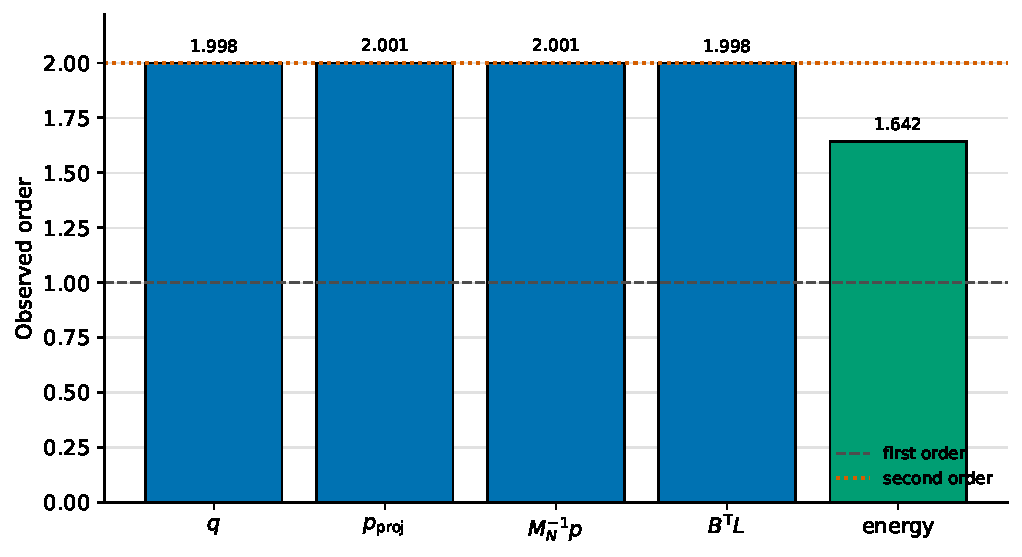
\includegraphics[width=0.88\linewidth]{figures/fig_b0_r2_convergence_orders.pdf}
\caption{Observed convergence orders in the three-level time-discretization study of the canonical data contract. The orders range from \(1.64186\) to \(2.00088\) and all exceed one; these results do not establish BDF symplecticity or constitute numerical KAM certification.}
\label{fig:b0-r2-convergence-orders}
\end{figure}

These results show that the current canonical data contract meets the data-generation requirements for subsequent multi-amplitude sentinel experiments. Multi-amplitude statistics, construction of the full 96-trajectory data set, and the full P2 model comparison will be reported in subsequent experiments. The present results do not establish that CHNN is generally superior to Real HNN on that full task.

\subsection{Open-port and high-fidelity numerical-validation plan}\label{sec:numerical-6-4}

The open-port branch will compare state-prediction error, componentwise generalized-force errors, power-balance residual, dissipation-sign violation rate, port leakage, and long-time trajectory error under paired operating conditions and ablations. These comparisons are designed to test the identifiability of conservative, dissipative, and externally applied forces. High-fidelity comparisons will quantify the discrepancy of the primary Kirchhoff model relative to Timoshenko-beam and solid models. The corresponding computations remain to be carried out, so this section specifies methods and metrics without asserting model superiority.

\subsection{High-order error certificates and numerical KAM validation}\label{sec:numerical-6-5}

Numerical KAM analysis requires a specified principal modal order, integrable reference system, and normal-form coefficients, together with the frequency-map nondegeneracy margin, a finite-order Diophantine margin, a high-order or analytic error certificate, the symplectic-map defect, a step-size nonresonance condition, and invariant-torus residuals. Numerical certification can be discussed only after the total error and the selected KAM threshold are expressed in the same norm. The present canonical-closure and time-step-convergence results do not constitute numerical KAM certification, and no invariant torus has yet been obtained.

\subsection{Parameter continuation, model discrepancy, and safe operating domain}\label{sec:numerical-6-6}

Subsequent studies will perform continuation in magnetic-field strength, insertion speed, flow velocity, contact clearance, and material parameters while reporting structural responses, port quantities, and discrepancies between reduced and high-fidelity models. A complete engineering safe domain must additionally incorporate open-port power exchange, peak contact response, high-fidelity discrepancy, and uncertainty propagation; it cannot be identified with the theoretical guarantee domain of the conservative KAM backbone. Because these computations have not yet been instantiated, this work does not claim an engineering safe domain.
